\documentclass{standalone}
\usepackage{tikz}
\usetikzlibrary{angles,quotes}
\begin{document}
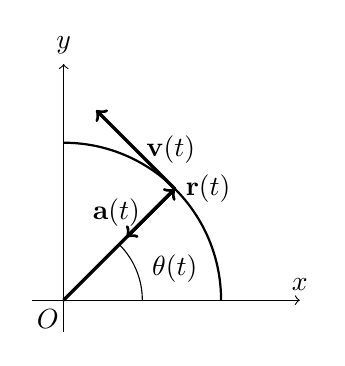
\begin{tikzpicture}[scale=2]
    \node[below] at(-0.1, 0) {$O$};
    \draw[->] (-0.2,0)--(1.5,0)coordinate(x)node[above]{$x$};
    \draw[->] (0,-0.2)--(0,1.5)node[above]{$y$};

    \draw[thick](1,0)arc(0:90:1);
    \coordinate (r) at (0.707, 0.707);
    \coordinate (nu) at (0.4, 0.4);
    \coordinate (O) at(0,0);

    \draw[->,very thick] (O)--(r) node[right]{$\mathbf{r}(t)$};
    \draw[->,very thick] (r)--(0.207,1.207)node[midway, right]{$\mathbf{v}(t)$};
    \draw[->,very thick] (r)--(nu) node[midway, left]{$\mathbf{a}(t)$};

    \node[right] at(0.5,0.2){$\theta(t)$};
    \pic[draw, angle eccentricity=1.2, angle radius=1cm]{angle=x--O--r};
\end{tikzpicture}
\end{document}